\section{CAN bus physical layer}

This section specifies the CAN-based physical layer of UAVCAN.

Here and in the following parts of this section,
``CAN'' implies both CAN 2.0 and CAN FD, unless specifically noted otherwise.

\subsection{Physical connector specification}

The UAVCAN standard defines several connector types, targeted towards different application domains:
from highly compact systems to large deployments, from low-cost to safety-critical applications.

The table \ref{table:can_connector_summary} provides an overview of the currently defined connector types
for the CAN bus transport implementation.
Other connector types may be added in future revisions of the specification.

It is highly recommended to provide two identical parallel connectors for each CAN interface per device,
and not using \mbox{T-connectors}.
\mbox{T-connectors} should be avoided because they add another point of failure,
increase the stub length, weight, and often require more complex and expensive wiring harnesses.

\begin{UAVCANSimpleTable}{Standard CAN connector types}{l l l X}\label{table:can_connector_summary}
    Connector name & Base connector type & Bus power & Known compatible standards \\
    \textbf{UAVCAN D-Sub} &
    Generic D-Subminiature DE-9 &
    24 V, 3 A &
    De-facto standard connector for CAN, supported by many current specifications. \\

    \textbf{UAVCAN M8} &
    Generic M8 5-circuit B-coded &
    24 V, 3 A &
    CiA 103 (CANopen) \\

    \textbf{UAVCAN Micro} &
    JST GH 4-circuit &
    5 V, 1 A &
    Dronecode Autopilot Connector Standard \\
\end{UAVCANSimpleTable}

\clearpage  % Enforce \clearpage because the text here is very graphics-heavy and may be hard to read otherwise
\subsubsection{UAVCAN D-Sub connector}

The UAVCAN D-Sub connector type is based upon, and compatible with, the D-Subminiature DE-9 CAN connector
(this is the most popular CAN connector type, in effect the de-facto industry standard).
This connector is fully compatible with CANopen and many other current specifications.
An example connector pair is pictured on the figures \ref{fig:can_uavcan_d_sub_connector_device}
and \ref{fig:can_uavcan_d_sub_connector_cable}.

{
\NoLeftSkip
\begin{UAVCANCompactTable}{X X}
    Advantages & Disadvantages \\
    \begin{itemize}
        \item Highest level of compatibility with the existing commercial off the shelf (COTS) hardware.
        Connectors, cables, termination plugs, and other components can be easily purchased from many different vendors.
        \item High-reliability options are available from multiple vendors.
        \item Low-cost options are available from multiple vendors.
        \item Both PCB mounted and panel mounted types are available.
    \end{itemize}
    &
    D-Subminiature connectors are the largest connector type defined by UAVCAN.
    Due to its significant size and weight, it may be unsuitable for many vehicular applications.
\end{UAVCANCompactTable}
}

The UAVCAN D-Sub connector is based on the industry-standard \textbf{D-Sub DE-9} (9-circuit) connector type.
Devices are equipped with the male plug connector type mounted on the panel or on the PCB,
and the cables are equipped with the female socket connectors on both ends
(see the figures \ref{fig:can_uavcan_d_sub_connector_device} and \ref{fig:can_uavcan_d_sub_connector_cable}).

If the device uses two parallel connectors per CAN bus interface (as recommended),
then all of the lines of the paired connectors,
including those that are not used by the current specification,
must be interconnected one to one.
This will ensure compatibility with future revisions of the specification that make use of
currently unused circuits of the connector.

The CAN physical layer standard that can be used with this connector type is
ISO 11898-2\footnote{Also known as \emph{high-speed CAN}.}.

Devices that deliver power to the bus are required to provide 23.0--30.0 V on the bus power line, 24 V nominal.
The maximum current draw is up to 3 A per connector.

Devices that are powered from the bus should expect 18.0--30.0 V on the bus power line.
The maximum recommended current draw from the bus is 0.5 A per device.

The table \ref{table:can_uavcan_d_sub_pinout} documents the pinout specification for the
UAVCAN D-Sub connector type.
The provided pinout, as has been indicated above, is the de-facto industry standard for the CAN bus.
Note that the signals ``CAN High'' and ``CAN Low'' must belong to the same twisted pair.
Usage of twisted or flat wires for all other signals remains at the discretion of the implementer.

\begin{UAVCANSimpleTable}{UAVCAN D-Sub connector pinout}{|l l X|}\label{table:can_uavcan_d_sub_pinout}
    \# & Function           & Note \\
    1  &                    &  \\
    2  & CAN low            & Twisted with ``CAN high'' (pin 7). \\
    3  & CAN ground         & Must be interconnected with ``Ground'' (pin 6) within the device. \\
    4  &                    &  \\
    5  & CAN shield         & Optional. \\
    6  & Ground             & Must be interconnected with ``CAN ground'' (pin 3) within the device. \\
    7  & CAN high           & Twisted with ``CAN low'' (pin 2). \\
    8  &                    &  \\
    9  & Bus power supply   & 24 V nominal. See the power supply requirements. \\
\end{UAVCANSimpleTable}

\begin{figure}[hbt]
    \centering
    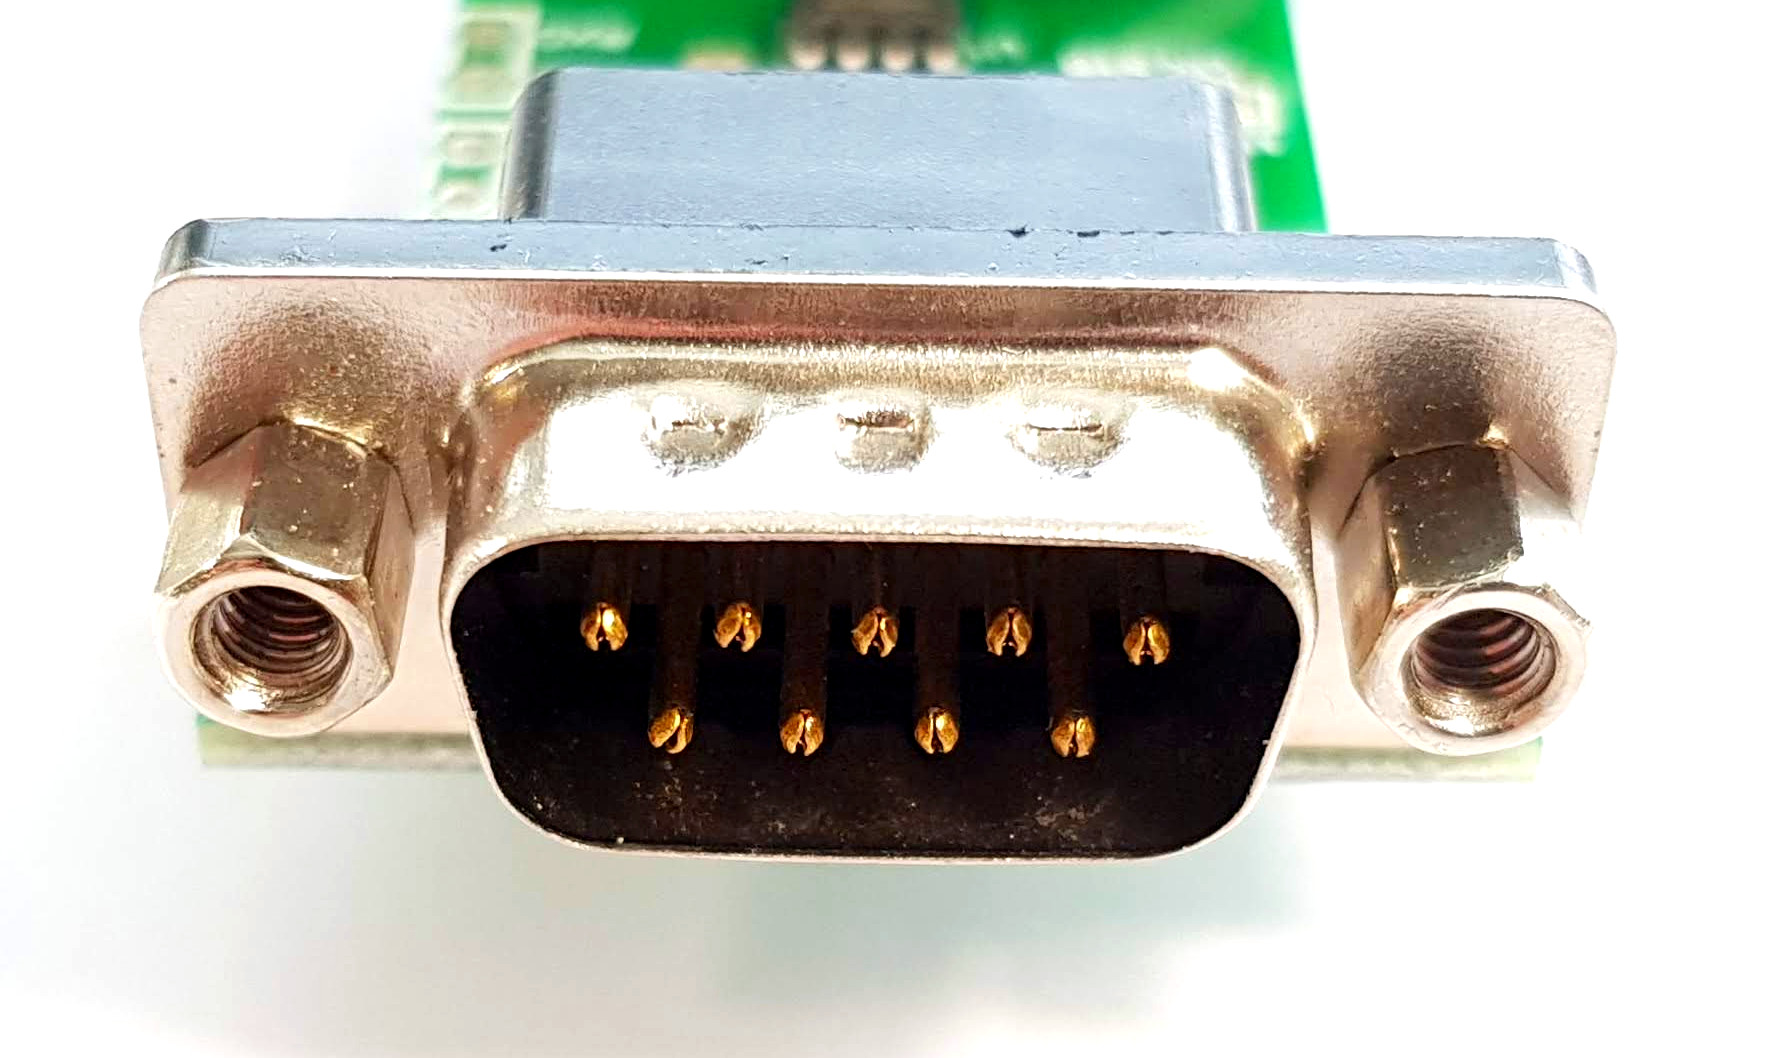
\includegraphics[width=0.6\textwidth]{physical_layer/de-9_connector_male_plug}
    \caption{UAVCAN D-Sub device connector example.
    \label{fig:can_uavcan_d_sub_connector_device}}
\end{figure}

\begin{figure}[hbt]
    \centering
    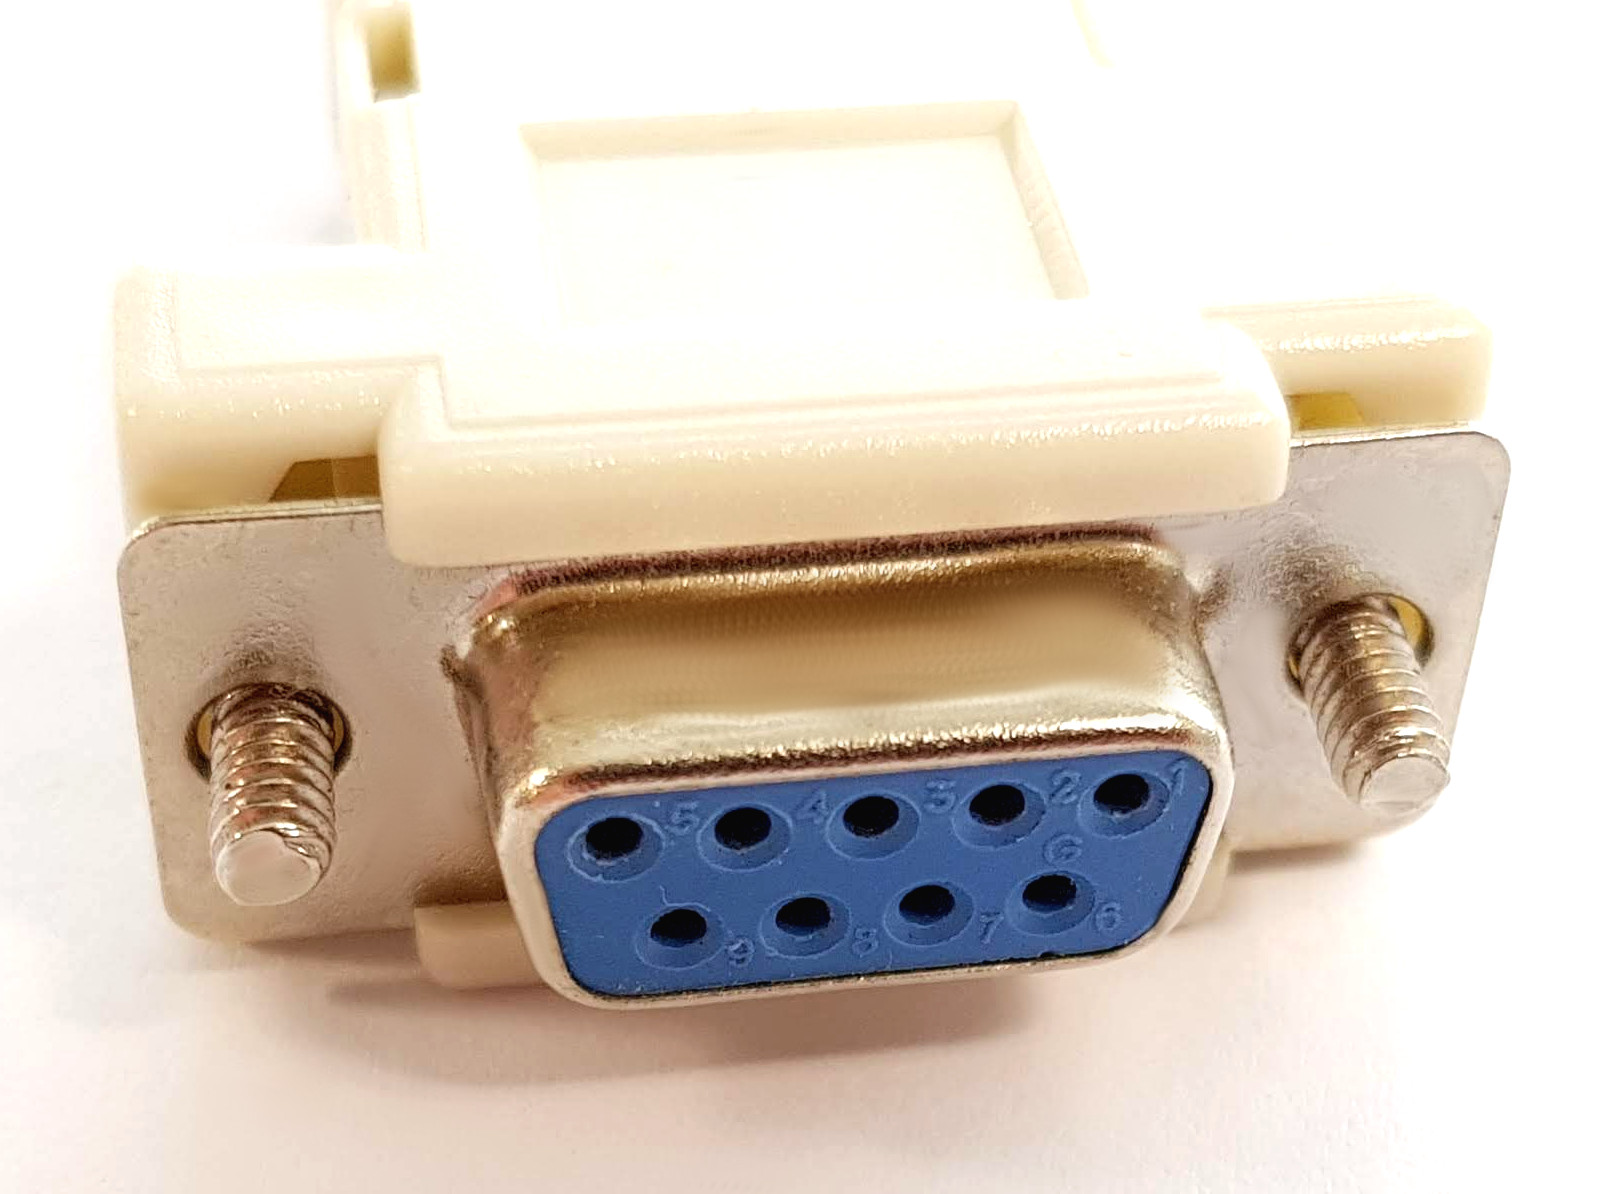
\includegraphics[width=0.6\textwidth]{physical_layer/de-9_cable_female_socket}
    \caption{UAVCAN D-Sub cable connector example.
    \label{fig:can_uavcan_d_sub_connector_cable}}
\end{figure}

\clearpage  % Enforce \clearpage because the text here is very graphics-heavy and may be hard to read otherwise
\subsubsection{UAVCAN M8 connector}

The UAVCAN M8 connector type is based on the generic circular M8 connector type,
shown on the figure \ref{fig:can_uavcan_m8_connector_example}.
This is a popular industry-standard connector, and there are many vendors that manufacture compatible components:
connectors, cables, termination plugs, T-connectors, and so on.
The pinning, physical layer, and supply voltages used in this connector type are compatible with CiA 103 (CANopen)
and some other CAN bus standards.

The M8 connector is preferred for most UAVCAN applications (it should be the default choice,
except when there are specific reasons to select another standard connector type).

{
\NoLeftSkip
\begin{UAVCANCompactTable}{X X}
    Advantages & Disadvantages \\
    \begin{itemize}
        \item Compatibility with existing COTS hardware.
        Connectors, cables, termination plugs, and other components can be purchased from many different vendors.
        \item High-reliability options are available from multiple vendors.
        \item Low-cost options are available from multiple vendors.
        \item Reasonably compact. M8 connectors are much smaller than D-Sub.
        \item PCB mounted and panel mounted types are available.
    \end{itemize}
    &
    \begin{itemize}
        \item M8 connectors may be a poor fit for applications that have severe weight and space constraints.
        \item The level of adoption in the industry is noticeably lower than that of the D-Sub connector type.
    \end{itemize}
\end{UAVCANCompactTable}
}

The UAVCAN M8 connector is based on the industry-standard \textbf{circular M8 B-coded 5-circuit} connector type.
Devices are equipped with the male plug connector type
mounted on the panel or on the PCB, and the cables are equipped with the female socket connectors on both ends
(see the figure \ref{fig:can_uavcan_m8_connector_example}).
\emph{Do not confuse A-coded and B-coded M8 connectors -- they are not mutually compatible}.

The CAN physical layer standard that can be used with this connector type is
ISO 11898-2\footnote{Also known as \emph{high-speed CAN}.}.

Devices that deliver power to the bus are required to provide 23.0--30.0 V on the bus power line, 24 V nominal.
The maximum current draw is up to 3 A per connector.

Devices that are powered from the bus should expect 18.0--30.0 V on the bus power line.
The maximum recommended current draw from the bus is 0.5 A per device.

The table \ref{table:can_uavcan_m8_pinout} documents the pinout specification for the UAVCAN M8 connector type.
The provided pinout, as indicated above, is compatible with the CiA 103 specification (CANopen).
Note that the wires ``CAN high'' and ``CAN low'' should be a twisted pair.

\begin{UAVCANSimpleTable}{UAVCAN M8 connector pinout}{|l l X|}\label{table:can_uavcan_m8_pinout}
    \# & Function           & Note \\
    1  & Bus power supply   & 24 V nominal. See the power supply requirements. \\
    2  & CAN shield         & Optional. \\
    3  & CAN high           & Twisted with ``CAN low'' (pin 4). \\
    4  & CAN low            & Twisted with ``CAN high'' (pin 3). \\
    5  & Ground             & \\
\end{UAVCANSimpleTable}

\begin{figure}[hbt]
    \centering
    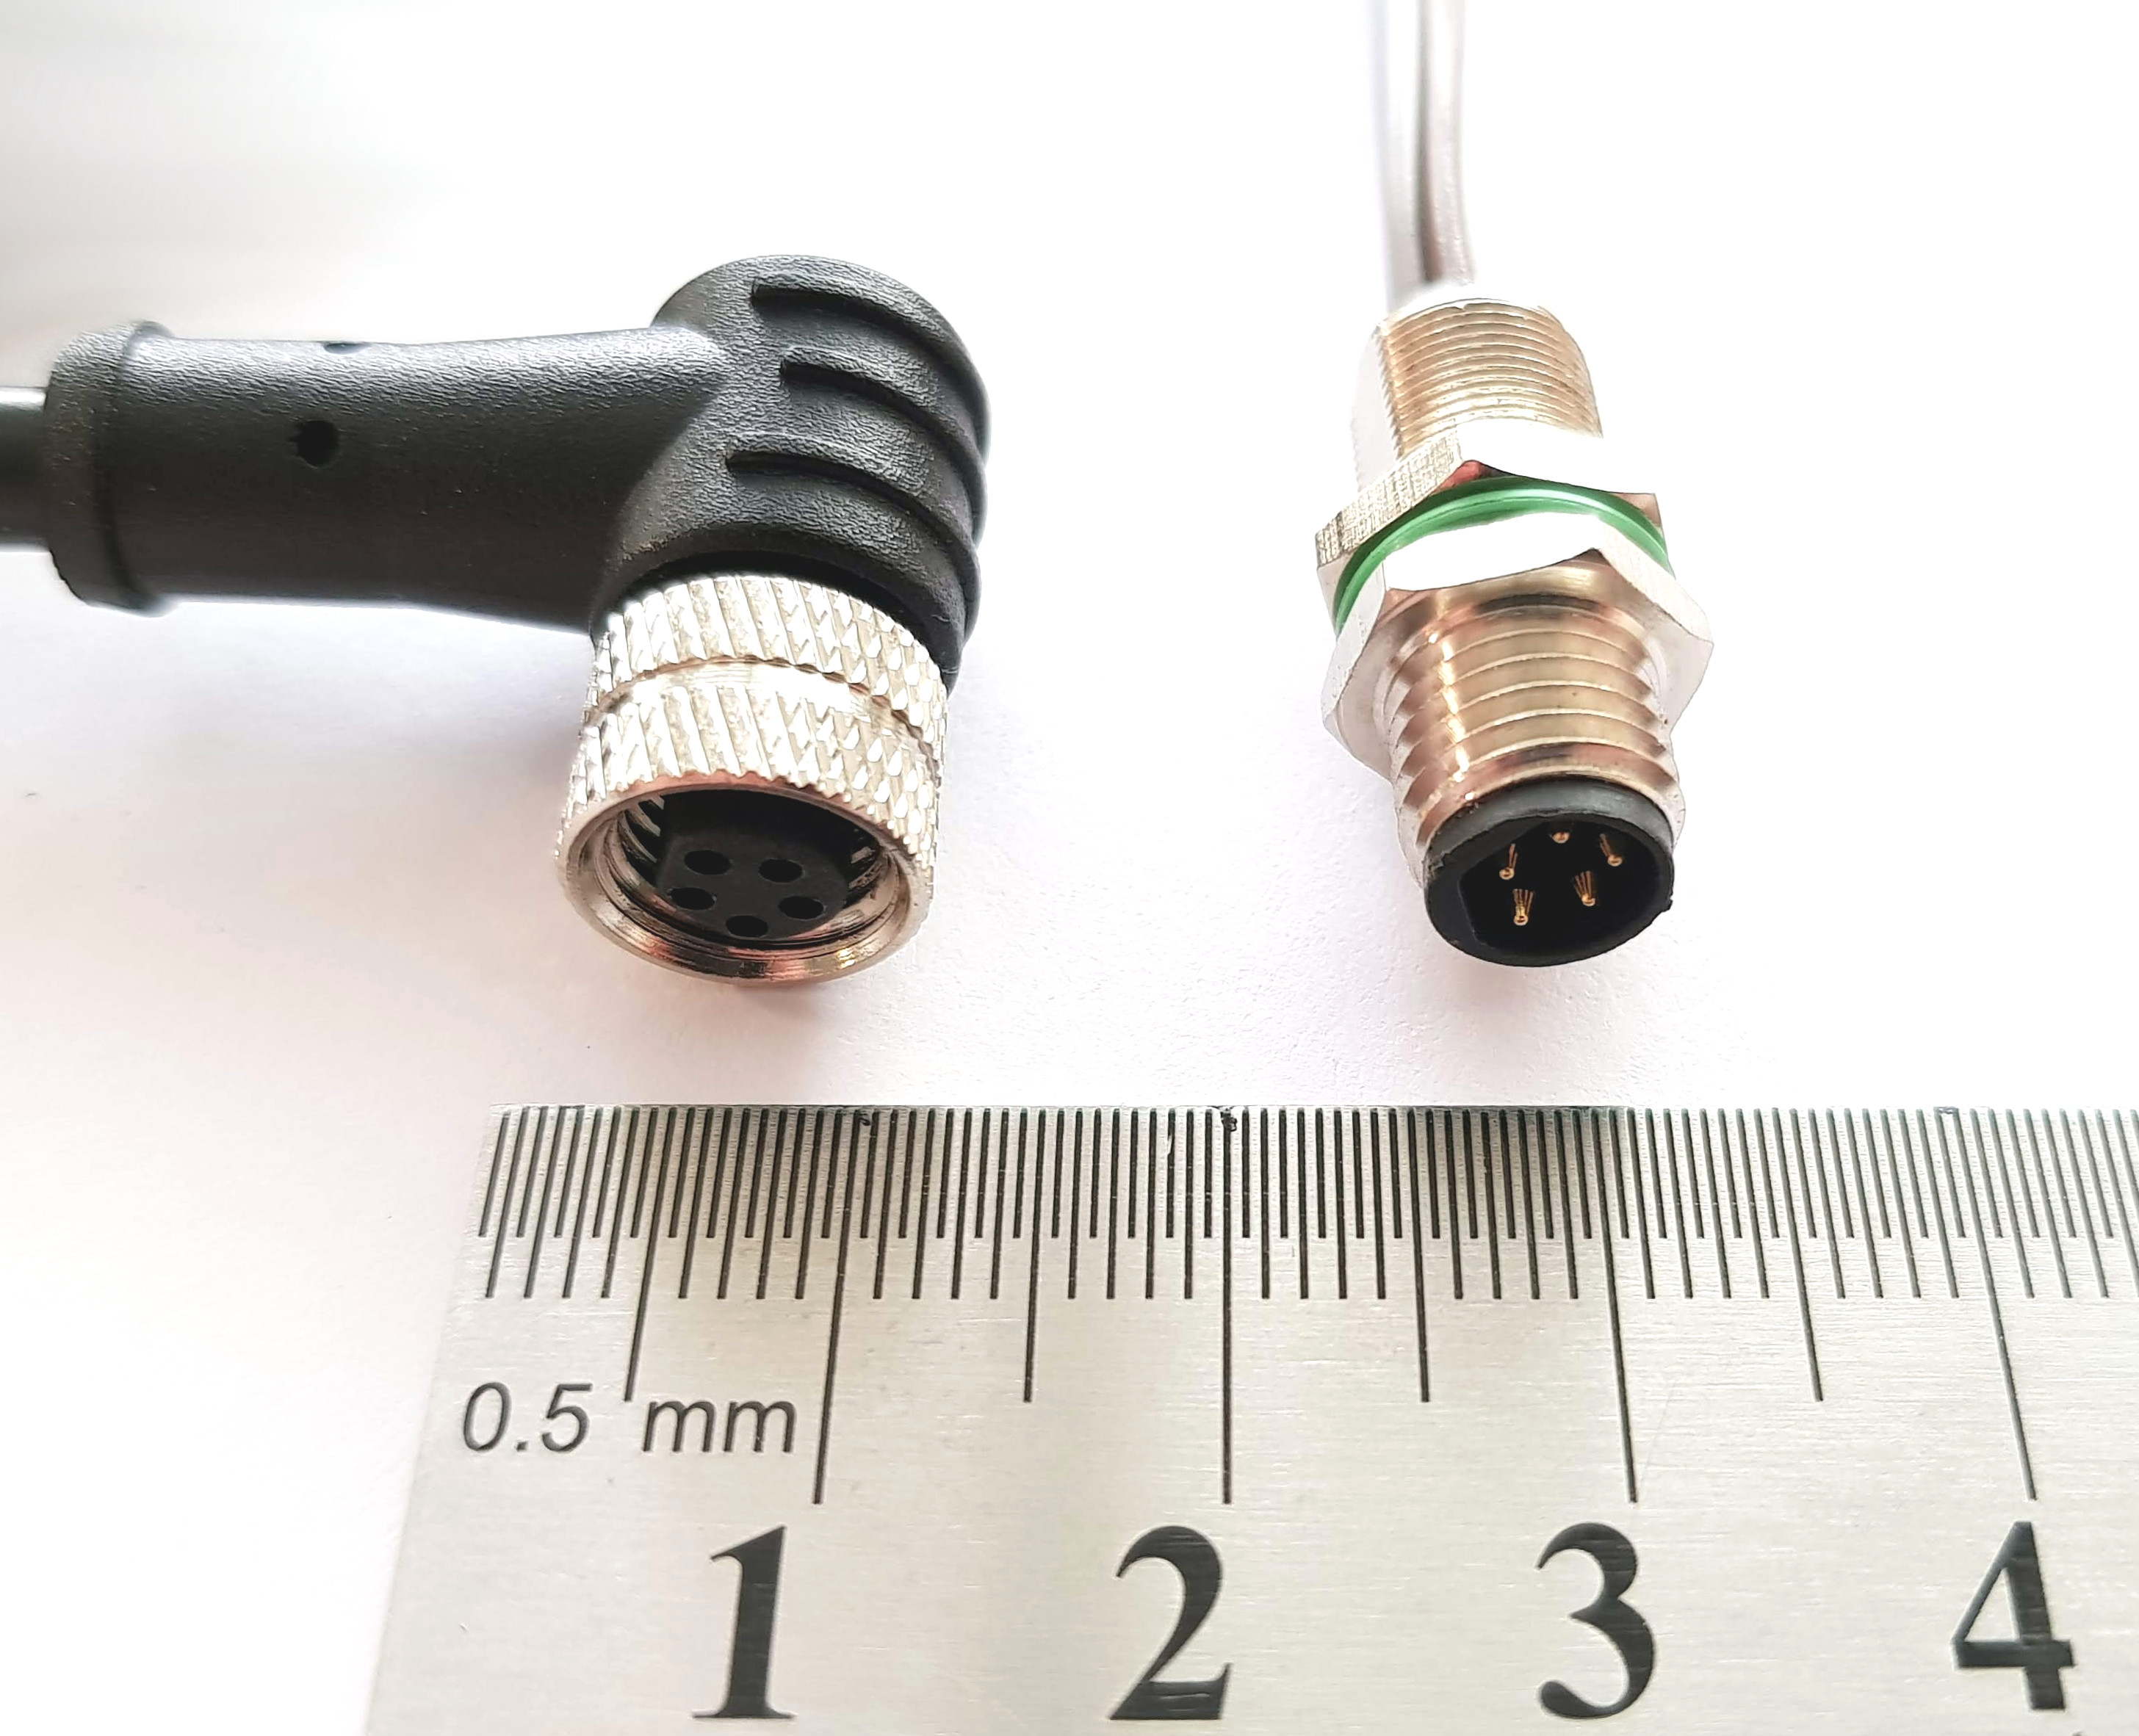
\includegraphics[width=0.7\textwidth]{physical_layer/m8_connector_pair_female_socket_male_plug}\\
    Example connectors: female socket cable (left) and male plug device connector (right).
    Different connector types are available from various vendors: PCB mounted, panel mounted;
    straight cables, angled cables, etc.
    \caption{UAVCAN M8 connector pair example.
    \label{fig:can_uavcan_m8_connector_example}}
\end{figure}

\begin{figure}[hbt]
    \centering
    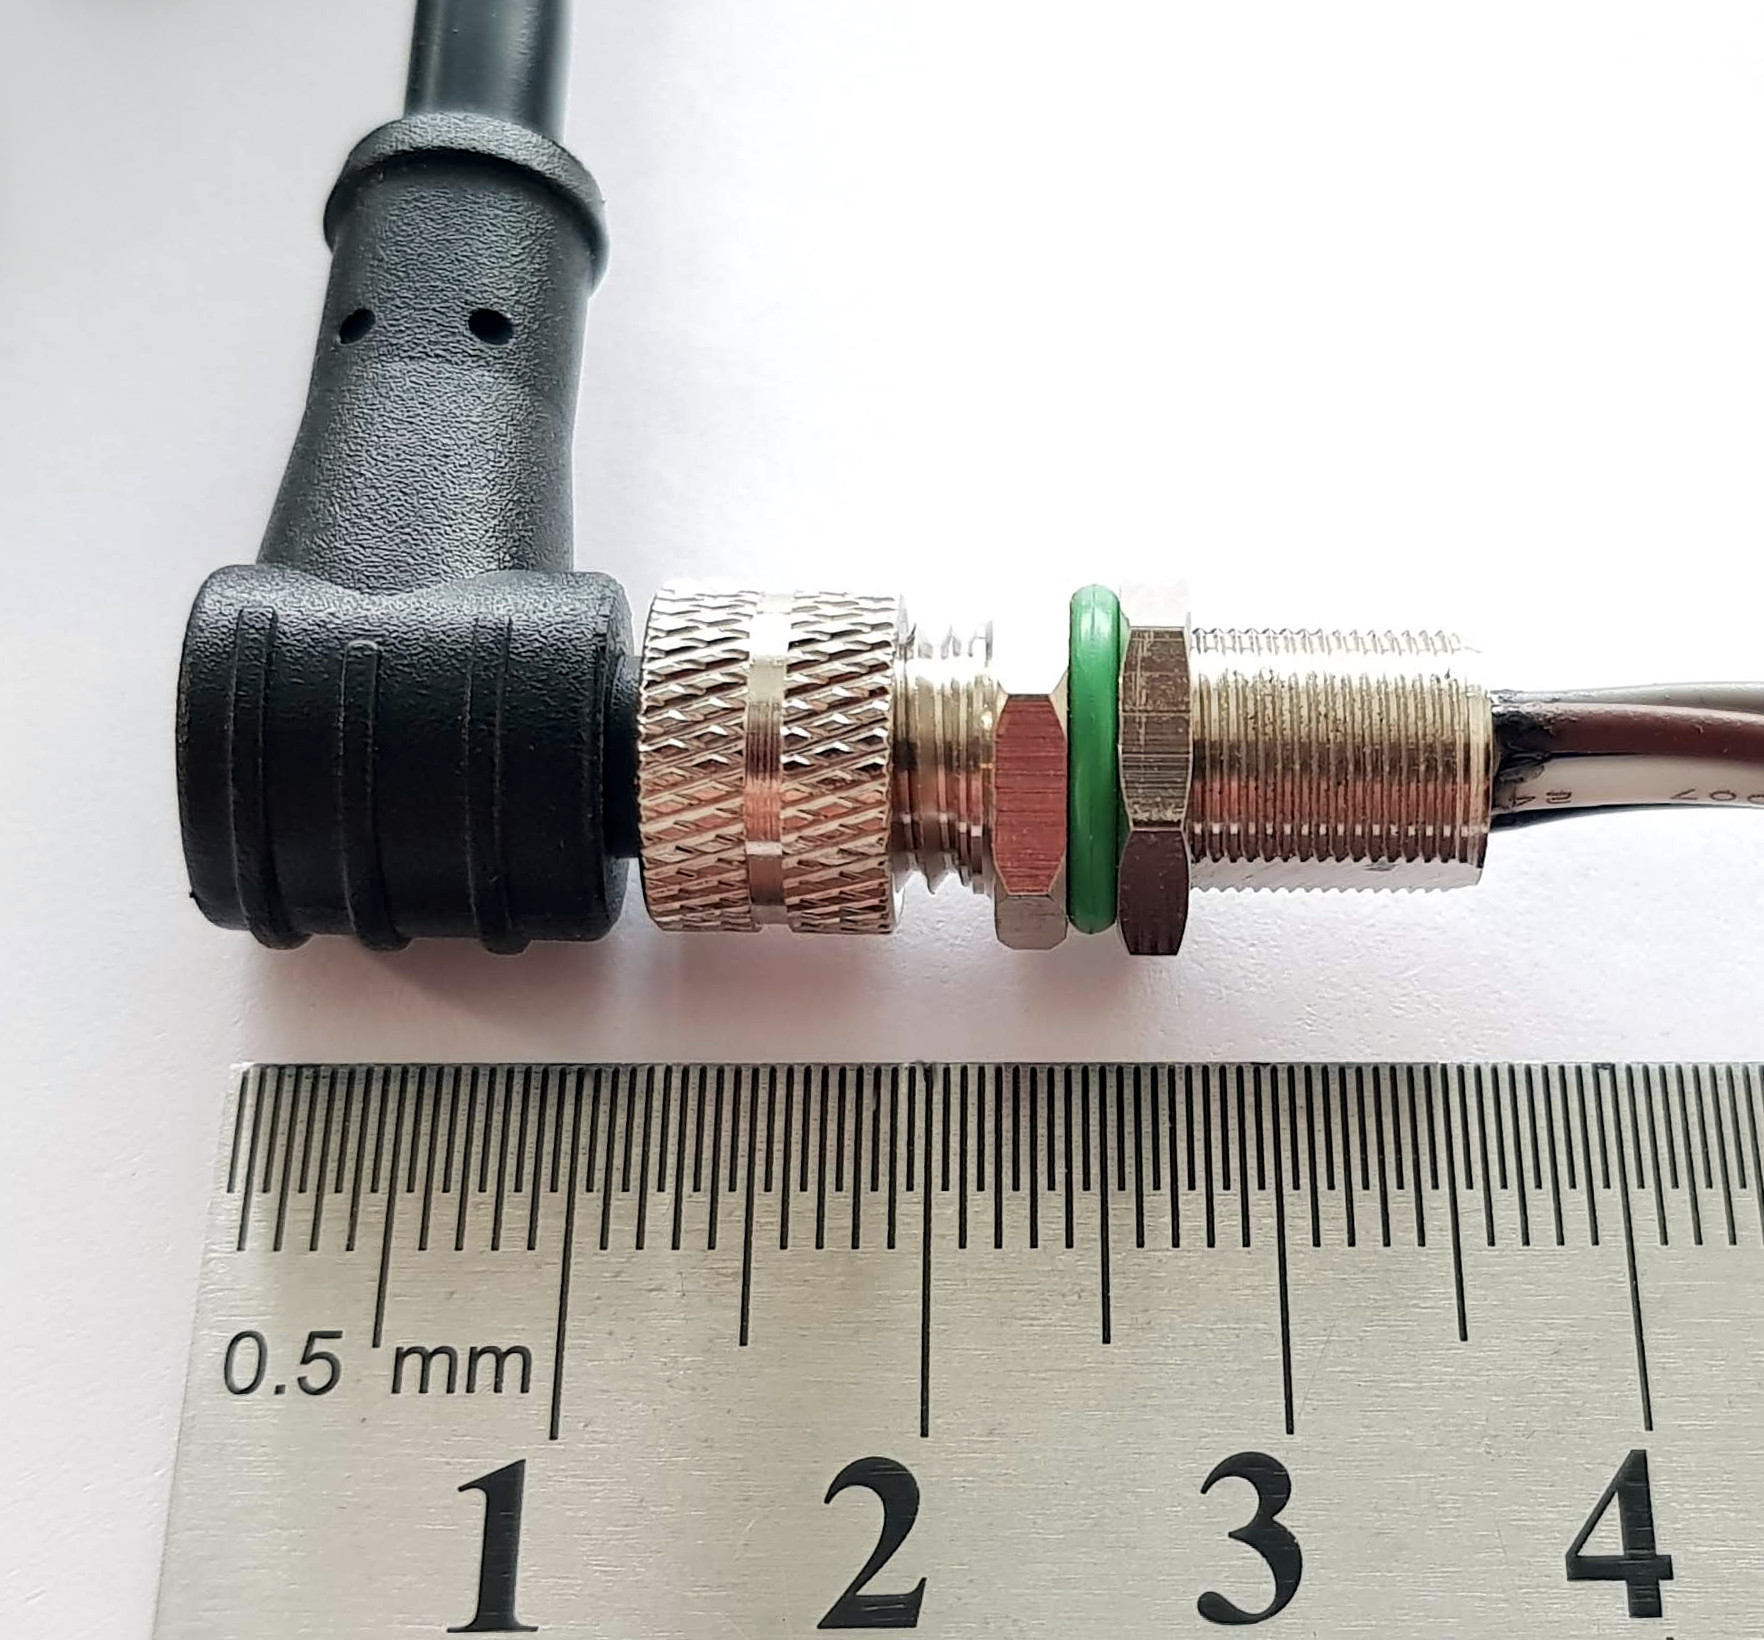
\includegraphics[width=0.7\textwidth]{physical_layer/m8_connector_pair_assembled}
    \caption{UAVCAN M8 assembled connector pair example.}
\end{figure}

\clearpage  % Enforce \clearpage because the text here is very graphics-heavy and may be hard to read otherwise
\subsubsection{UAVCAN Micro connector}

The UAVCAN Micro connector is intended for weight- and space-sensitive applications.
It is a board-level connector, meaning that it can be installed on the PCB rather than on the panel.
An example is shown on the figure \ref{fig:can_uavcan_micro_connector_example}.

The Micro connector is compatible with the Dronecode Autopilot Connector Standard.
This connector type is recommended for small UAV and nanosatellites.
It is also the recommended connector for attaching external panel-mounted connectors
(such as the M8 or D-Sub types) to the PCB inside the enclosure.

{
\NoLeftSkip
\begin{UAVCANCompactTable}{X X}
    Advantages & Disadvantages \\
    \begin{itemize}
        \item Extremely compact, low-profile. The PCB footprint is under 9$\times$5 millimeters.
        \item Secure positive lock ensures that the connection will not self-disconnect when exposed to vibrations.
        \item Low-cost, easy to stock.
    \end{itemize}
    &
    \begin{itemize}
        \item Board-level connections only. No panel-mounted options available.
        \item No shielding available.
        \item Not suitable for safety-critical hardware.
    \end{itemize}
\end{UAVCANCompactTable}
}

The UAVCAN Micro connector is based on the proprietary \textbf{JST GH 4-circuit} connector type.
Beware that the top-entry type is not PCB footprint-compatible with the side-entry type --
its pin ordering is reversed.
The wire-side pinout, however, is compatible, so both types can be used interchangeably as long
as their PCB footprints are correct.

The suitable cable types are flat or twisted pair \#30 to \#26 AWG,
outer insulation diameter 0.8--1.0 mm, multi-strand.
Non-twisted (flat) cables can only be used in very small deployments free of significant
EMI\footnote{Electromagnetic interference.};
otherwise, reliable functioning of the bus cannot be guaranteed.

The CAN physical layer standard that can be used with this connector type is ISO 11898-2.

Devices that deliver power to the bus are required to provide 5.0--5.5 V on the bus power line.
The anticipated current draw is up to 1 A per connector.

Devices that are powered from the bus should expect 4.0--5.5 V on the bus power line.
The maximum recommended current draw from the bus is 0.5 A per device.

The table \ref{table:can_uavcan_micro_pinout} documents the pinout specification for the UAVCAN M8 connector type.
The provided pinout, as indicated above, is compatible with the Dronecode Autopilot Connector Standard.
Note that the wires ``CAN high'' and ``CAN low'' should be a twisted pair.

\begin{UAVCANSimpleTable}{UAVCAN Micro connector pinout}{|l l X|}\label{table:can_uavcan_micro_pinout}
    \# & Function           & Note \\
    1  & Bus power supply   & 5 V nominal. See the power supply requirements. \\
    2  & CAN high           & Should be twisted with ``CAN low'' (pin 3). \\
    3  & CAN low            & Should be twisted with ``CAN high'' (pin 2). \\
    4  & Ground             & \\
\end{UAVCANSimpleTable}

\begin{figure}[hbt]
    \centering
    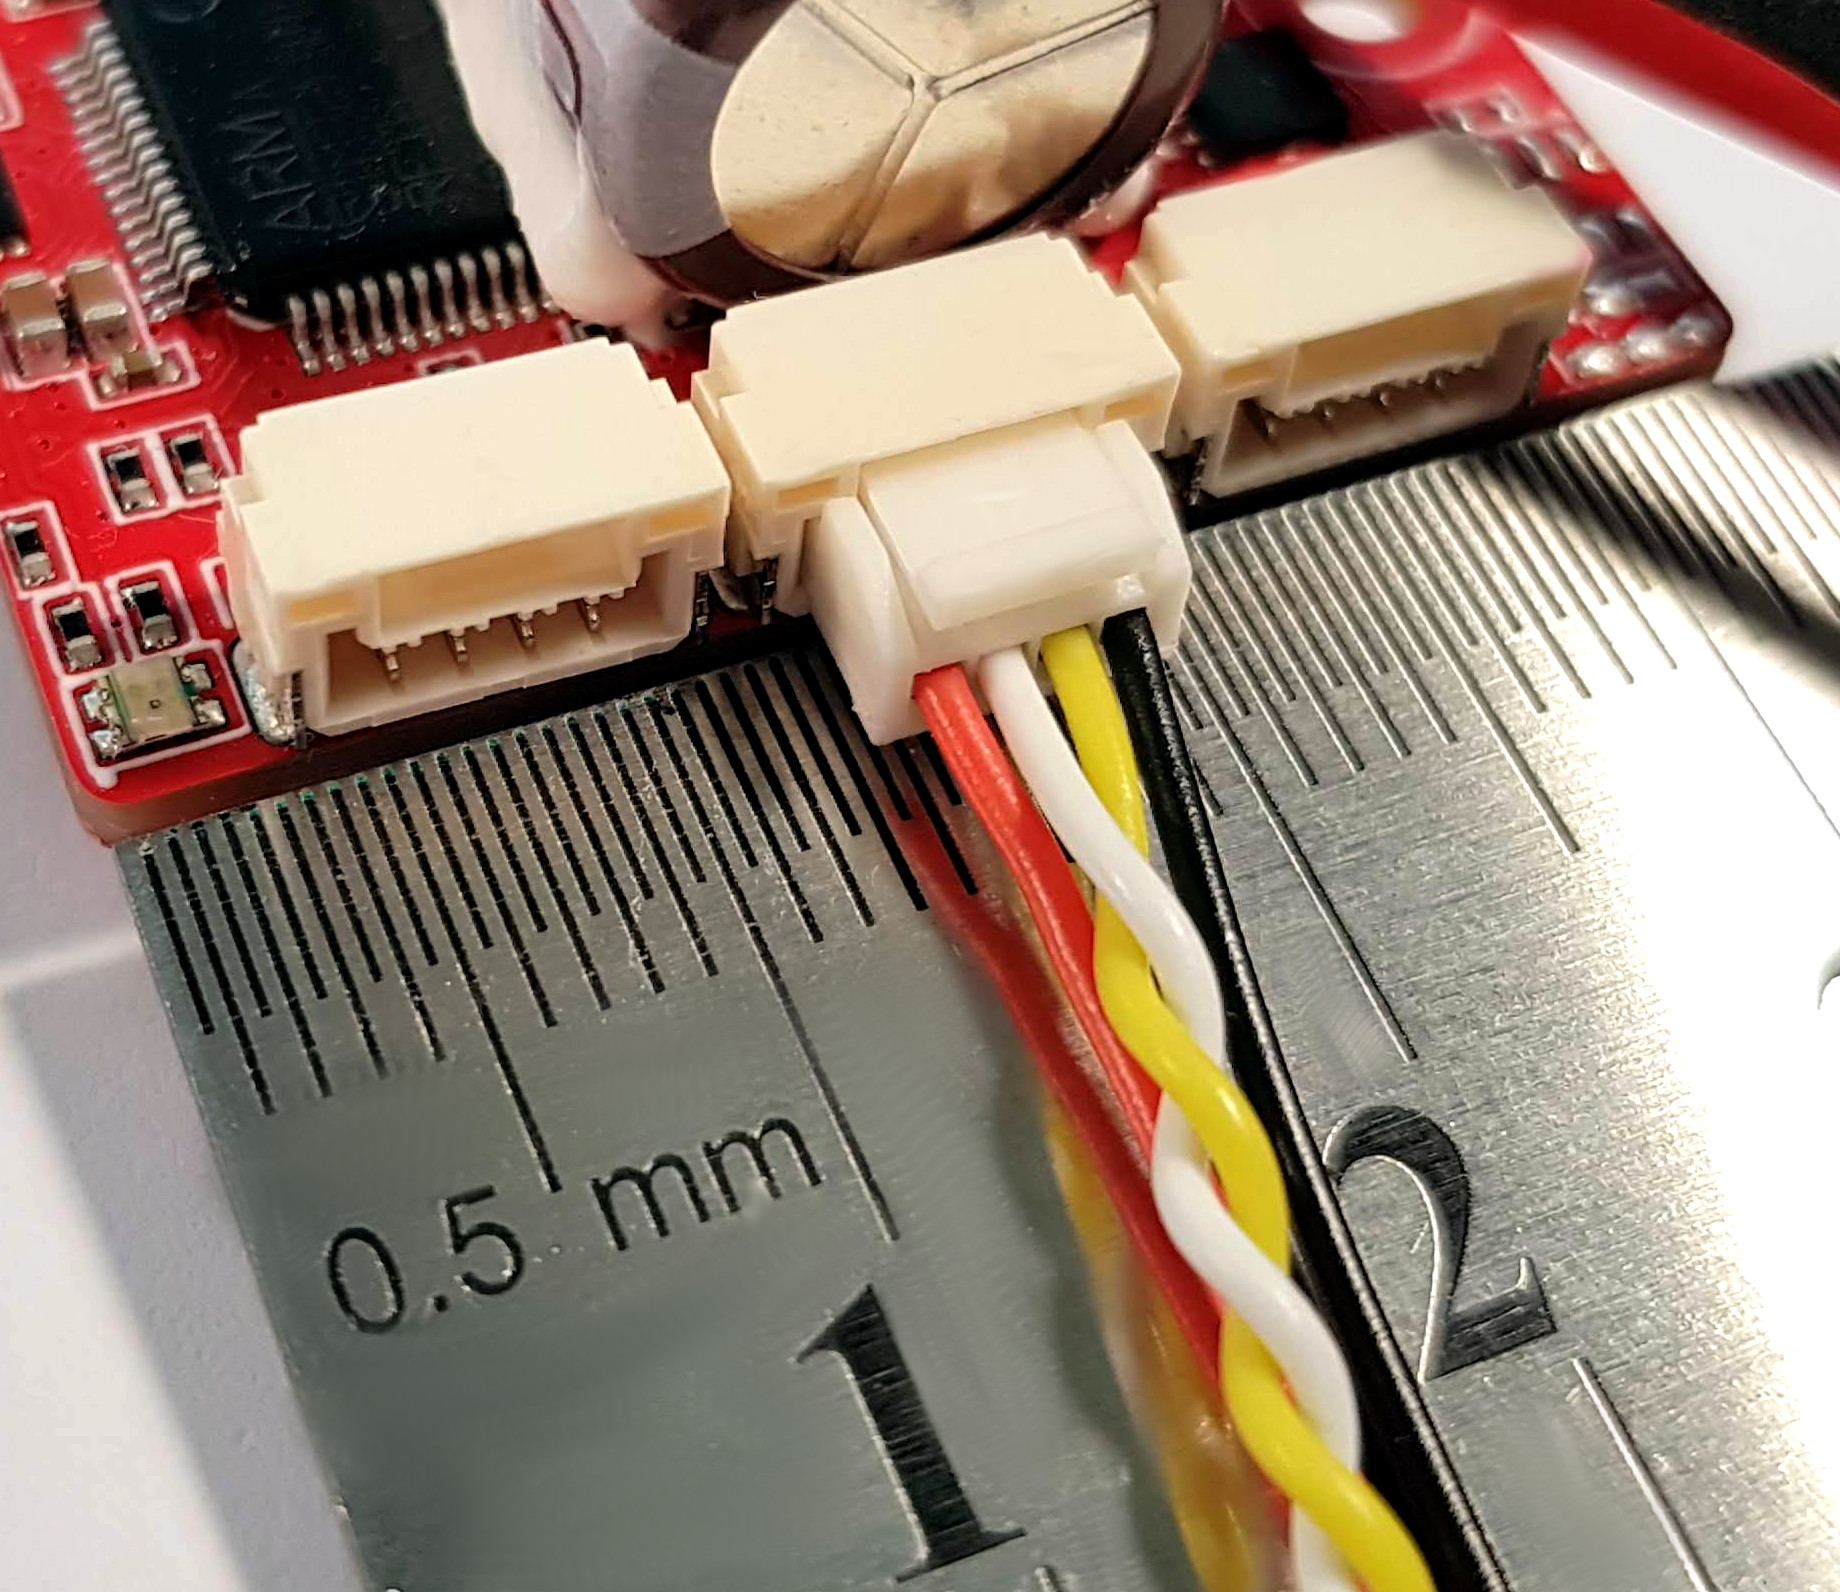
\includegraphics[width=0.7\textwidth]{physical_layer/jst_gh_connectors}
    \caption{UAVCAN Micro right-angle connectors with a twisted pair patch cable connected.
    \label{fig:can_uavcan_micro_connector_example}}
\end{figure}

\begin{figure}[hbt]
    \centering
    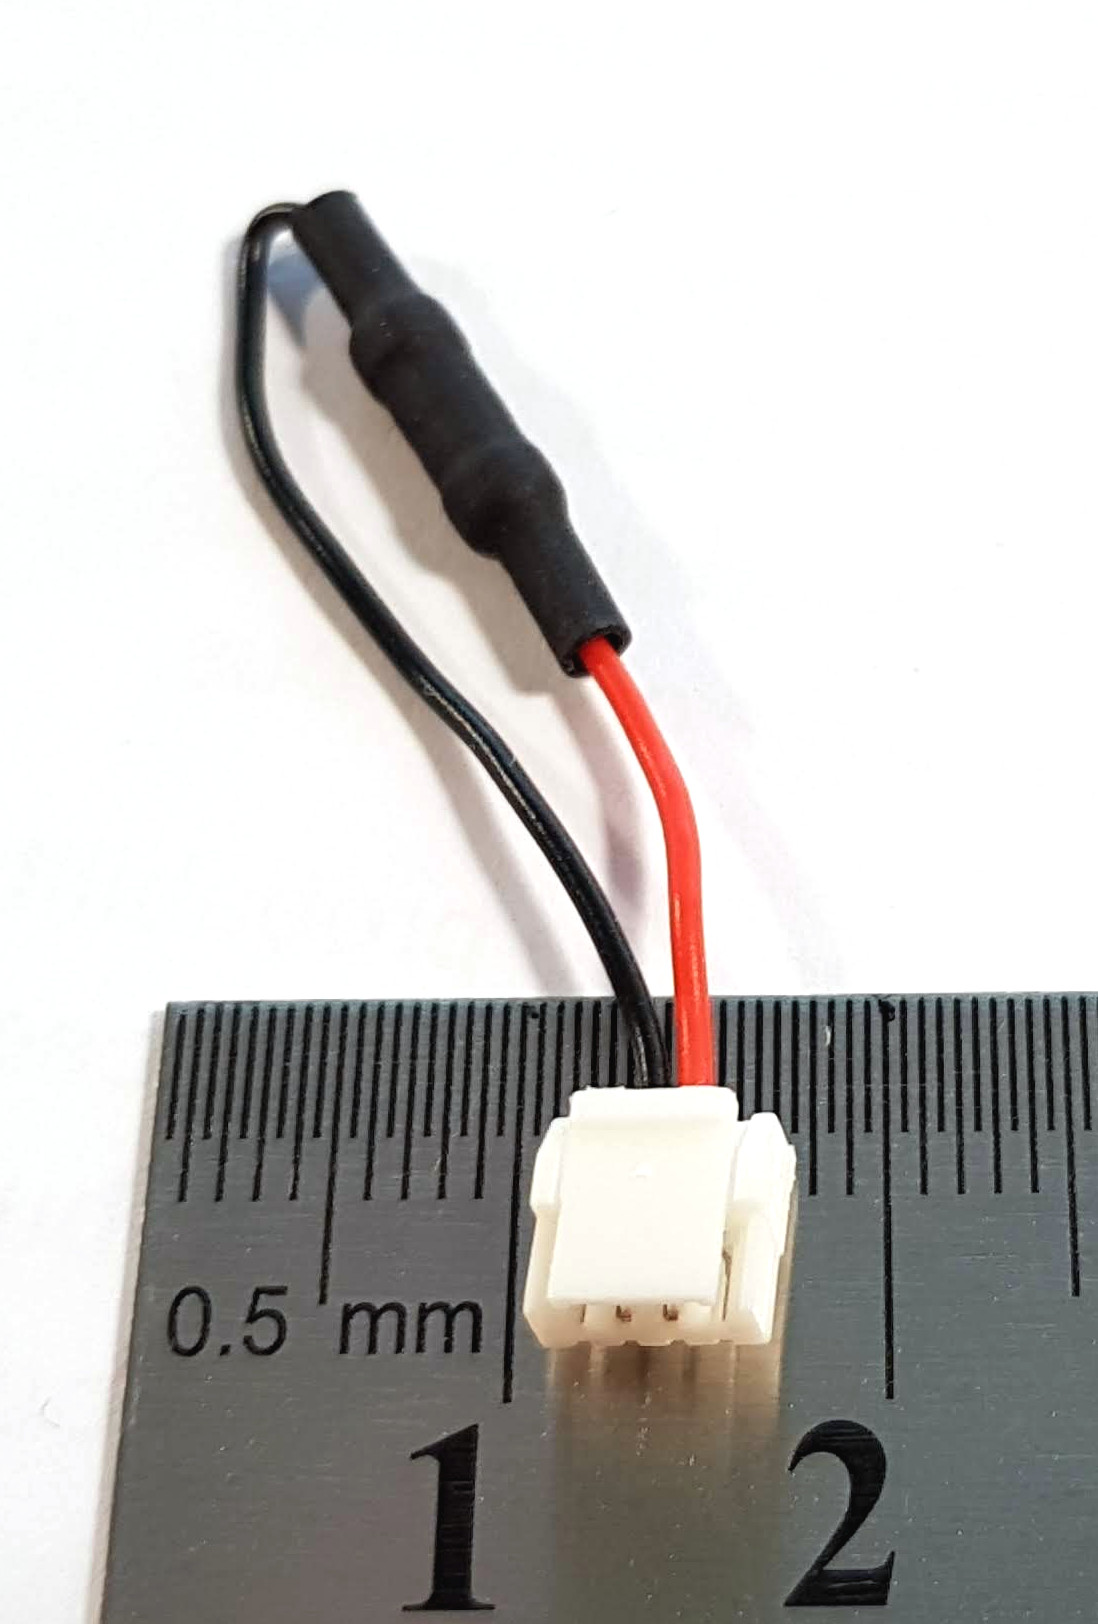
\includegraphics[width=0.4\textwidth]{physical_layer/jst_gh_termination_plug}
    \caption{UAVCAN Micro CAN bus termination plug.}
\end{figure}

\clearpage  % Enforce \clearpage because the text here is very graphics-heavy and may be hard to read otherwise
\subsection{CAN bus physical layer parameters}

As can be seen from the rest of the specification,
UAVCAN is mostly agnostic of the parameters of the physical layer.
However, vendors should follow the recommendations provided in this section
to maximize the cross-vendor compatibility.

\subsubsection{CAN 2.0}

This section is dedicated to the legacy CAN 2.0 protocol.

The table \ref{table:can_2.0_phy_parameters} lists the standard parameters of the CAN PHY for
ISO 11898-2.
The estimated bus length limits are based on the assumption that the propagation delay does not exceed 5 ns/m,
not including additional delay times of CAN transceivers and other components.

\begin{UAVCANSimpleTable}{Standard CAN 2.0 PHY parameters}{|X[c] X[c] X[c] X[c] X[c]|}
    Bit rate [kbit/s] &
    Valid range for location of sample point [\%] &
    Recommended location of sample point [\%] &
    Maximum bus length [m] &
    Maximum stub length [m] \label{table:can_2.0_phy_parameters} \\

    1000    & 75 to 90  & 87.5  & 40    & 0.3 \\
     500    & 85 to 90  & 87.5  & 100   & 0.3 \\
     250    & 85 to 90  & 87.5  & 250   & 0.3 \\
     125    & 85 to 90  & 87.5  & 500   & 0.3 \\
\end{UAVCANSimpleTable}

Designers are encouraged to implement CAN auto bit rate detection when applicable.
Please refer to the CiA 801 application note for the recommended practices.

UAVCAN allows the use of a simple bit time measuring approach,
as it is guaranteed that any functioning UAVCAN network will always exchange node status messages,
which can be expected to be published at a rate no lower than 1 Hz,
and that contain a suitable alternating bit pattern in the CAN ID field.
Please refer to the chapter \ref{sec:application_layer} for details.

\subsubsection{CAN FD}

This section will be populated in a later revision of the document.
